	%%% LaTeX Template: Designer's CV
%%%
%%% Source: http://www.howtotex.com/
%%% Feel free to distribute this template, but please keep the referal to HowToTeX.com.
%%% Date: March 2012


%%%%%%%%%%%%%%%%%%%%%%%%%%%%%%%%%%%%%
% Document properties and packages
%%%%%%%%%%%%%%%%%%%%%%%%%%%%%%%%%%%%%
\documentclass[a4paper,12pt,final]{memoir}

% misc
\renewcommand{\familydefault}{bch}	% font
\pagestyle{empty}					% no pagenumbering
\setlength{\parindent}{0pt}			% no paragraph indentation

\usepackage[T1]{fontenc}
\usepackage[utf8]{inputenc}
% required packages (add your own)
\usepackage{flowfram}										% column layout
\usepackage[top=1cm,left=1cm,right=1cm,bottom=1cm]{geometry}% margins
\usepackage{graphicx}										% figures
\usepackage{url}											% URLs
\usepackage[usenames,dvipsnames]{xcolor}					% color
\usepackage{multicol}										% columns env.
	\setlength{\multicolsep}{0pt}
\usepackage{paralist}										% compact lists
\usepackage{tikz}
\usepackage[francais]{babel}

%%%%%%%%%%%%%%%%%%%%%%%%%%%%%%%%%%%%%
% Create column layout
%%%%%%%%%%%%%%%%%%%%%%%%%%%%%%%%%%%%%
% define length commands
\setlength{\vcolumnsep}{\baselineskip}
\setlength{\columnsep}{\vcolumnsep}

% frame setup (flowfram package)
% left frame
\newflowframe{0.2\textwidth}{\textheight}{0pt}{0pt}[left]
	\newlength{\LeftMainSep}
	\setlength{\LeftMainSep}{0.2\textwidth}
	\addtolength{\LeftMainSep}{1\columnsep}
 
% small static frame for the vertical line
\newstaticframe{1.5pt}{\textheight}{\LeftMainSep}{0pt}
 
% content of the static frame
\begin{staticcontents}{1}
\hfill
\tikz{%
	\draw[loosely dotted,color=RoyalBlue,line width=1.5pt,yshift=0]
	(0,0) -- (0,\textheight);}%
\hfill\mbox{}
\end{staticcontents}
 
% right frame
\addtolength{\LeftMainSep}{1.5pt}
\addtolength{\LeftMainSep}{1\columnsep}
\newflowframe{0.7\textwidth}{\textheight}{\LeftMainSep}{0pt}[main01]


%%%%%%%%%%%%%%%%%%%%%%%%%%%%%%%%%%%%%
% define macros (for convience)
%%%%%%%%%%%%%%%%%%%%%%%%%%%%%%%%%%%%%
\newcommand{\Sep}{\vspace{1.5em}}
\newcommand{\SmallSep}{\vspace{0.5em}}

\newenvironment{AboutMe}
	{\ignorespaces\textbf{\color{RoyalBlue} About me}}
	{\Sep\ignorespacesafterend}
	
\newcommand{\CVSection}[1]
	{\Large\textbf{#1}\par
	\SmallSep\normalsize\normalfont}

\newcommand{\CVItem}[2]
	{\textbf{\color{RoyalBlue} #1 - {\small\color{black}#2}}\normalsize\normalfont}
	
%%%%%%%%%%%%%%%%%%%%%%%%%%%%%%%%%%%%%
% Begin document
%%%%%%%%%%%%%%%%%%%%%%%%%%%%%%%%%%%%%
\begin{document}

% Left frame
%%%%%%%%%%%%%%%%%%%%
\begin{figure}
	\hfill
	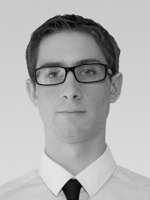
\includegraphics[width=0.6\columnwidth]{IMG_7936-Modifier_cv}
	\vspace{-7cm}
\end{figure}

\begin{flushright}\small
	Romain \textsc{Reignier} \\
	\url{romain.reignier@edu.supmeca.fr}  \\
	+33609521618 \\
	23 years old
\end{flushright}\normalsize
\framebreak


% Right frame
%%%%%%%%%%%%%%%%%%%%
\Huge\bfseries {\color{RoyalBlue} Romain \textsc{Reignier}} \\
\Large\bfseries  Student in Mechanical \& Robotics Engineering \\

\normalsize\normalfont

% % About me
% \begin{AboutMe}
% A young man a bit crazy !
% \end{AboutMe}

% Education
\CVSection{Education}

\CVItem{2013 - present, University of Toulon}{La Garde, Var}\\
Master Degree on Command \& Vision.
\SmallSep

\CVItem{2012 - present, Supmeca Engineering School}{La Garde, Var}\\
An engineering course focusing in mechanics with Robotics and Mecatronics.
\SmallSep

\CVItem{2009 - 2012, CPGE Victor Hugo}{Caen, Normandy}\\
Physics Sciences of Engineer (PSI).\\
Highly selective classes to prepare for the competitive exams to the Grandes Ecoles.
\SmallSep

\CVItem{2006 - 2009, Scientific Baccalaureat}{Valognes, Normandy}\\
Secondary School diploma in Sciences, specialized in Physics.
%With Honors.
\Sep

% Experience
\CVSection{Experience}
\CVItem{September 2013 - January 2014, R\&D CLAAS Tractor}{Vélizy, Yvelines}\\
Assistant engineer internship.\\
Work with the HVAC expert on the project to improve the AC of the K07 cabin.
Analysis of data from simulations and tests.
\SmallSep

\CVItem{January 2013, DCNS}{Cherbourg, Normandy}\\
Operator internship.\\
Work with numerical machine tools in the construction workshop of French nuclear
submarines.
\Sep

% % Skills
% \CVSection{Skills}
% \CVItem{Platforms}
% \begin{multicols}{3}
% \begin{compactitem}[\color{RoyalBlue}$\circ$]
% 	\item Lorem 
% 	\item Ipsum 
% \end{compactitem}
% \end{multicols}
% \SmallSep
% 
% \CVItem{Computer software}
% \begin{multicols}{3}
% \begin{compactitem}[\color{RoyalBlue}$\circ$]
% 	\item Lorem 
% 	\item Ipsum 
% 	\item Dolor 
% 	\item Sit 
% 	\item Amet
% 	\item Consectetur 
% 	\item Adipiscing 
% 	\item Elit
% 	\item \ldots
% \end{compactitem}
% \end{multicols}
% \Sep 
% 
% \CVSection{Something other}
% Lorem ipsum dolor sit amet, consectetur adipiscing elit. Vivamus vel bibendum metus. Proin rutrum pharetra molestie. Cras sollicitudin nulla nec leo lobortis in tristique purus pretium. Ut eu felis nulla. Pellentesque condimentum justo ut ligula feugiat nec facilisis tellus ultricies. Nullam sit amet dictum ipsum. Sed lacus neque, hendrerit eu rhoncus nec, pellentesque vitae sem.
% 
% \clearpage
% \framebreak
% \framebreak
% 
% \CVSection{Something else}
% Lorem ipsum dolor sit amet, consectetur adipiscing elit. Vivamus vel bibendum metus. Proin rutrum pharetra molestie. Cras sollicitudin nulla nec leo lobortis in tristique purus pretium. Ut eu felis nulla. Pellentesque condimentum justo ut ligula feugiat nec facilisis tellus ultricies. Nullam sit amet dictum ipsum. Sed lacus neque, hendrerit eu rhoncus nec, pellentesque vitae sem.
% \Sep
% 
% % References
% \CVSection{References}
% References upon request.

%%%%%%%%%%%%%%%%%%%%%%%%%%%%%%%%%%%%%
% End document
%%%%%%%%%%%%%%%%%%%%%%%%%%%%%%%%%%%%%
\end{document}
